The use of LLMs for automating test case generation has garnered significant attention. A number of methods have been proposed with the goal of improving code coverage. One such approach is HITS (Hierarchical Test Generation with Slicing) by Wang et al., which introduces a method of semantically dividing the target method into multiple “slices,” generating individual prompts for each, and integrating the resulting test cases \cite{hits}. This technique has demonstrated superior coverage compared to existing methods such as ChatUniTest, SymPrompt, and EvoSuite. Notably, it achieved an average statement coverage of 55.09\% and branch coverage of 48.12\% on complex Java methods.

However, these improvements in coverage come with trade-offs. The increase in prompt granularity and repeated interactions with the LLMs for each slice significantly inflates the total token count, leading to a sharp rise in API usage costs. This introduces a new challenge: balancing performance gains against the growing computational and financial overhead.

Another area gaining attention is the role of contextual information—specifically, in-code documentation such as comments and docstrings as shown blue lines in Fig.\ref{fig:ex_docstrings}—in influencing the performance of LLMs. Macke et al. quantitatively evaluated how the presence and accuracy of documentation affect LLMs comprehension and generation capabilities \cite{testing_the_effect_of_code_documentation}. Their findings revealed that incorrect documentation can severely degrade performance. For instance, when random, misleading comments contradicting the code were provided, GPT-3.5’s accuracy dropped to 22.1\%, with a increase in runtime errors. These results underscore the importance of not simply maximizing prompt content, but ensuring the accuracy and relevance of included information especially in the context of test case generation.

To address the token inflation problem, recent studies have focused on prompt compression and information extraction as strategies to streamline inputs. A representative example is LLMLingua-2 by Microsoft Research, which distills GPT-4’s knowledge into a lightweight language model that compresses natural language prompts by 2 to 5 times while retaining key information and maintaining task performance. Moreover, response times were accelerated by up to 2.9×, yielding efficiency gains in both cost and interaction latency. Although prompt compression has shown effectiveness in tasks such as natural language processing and code completion, its application in the domain of automated test case generation remains largely unexplored.

\begin{figure}
    \centering
    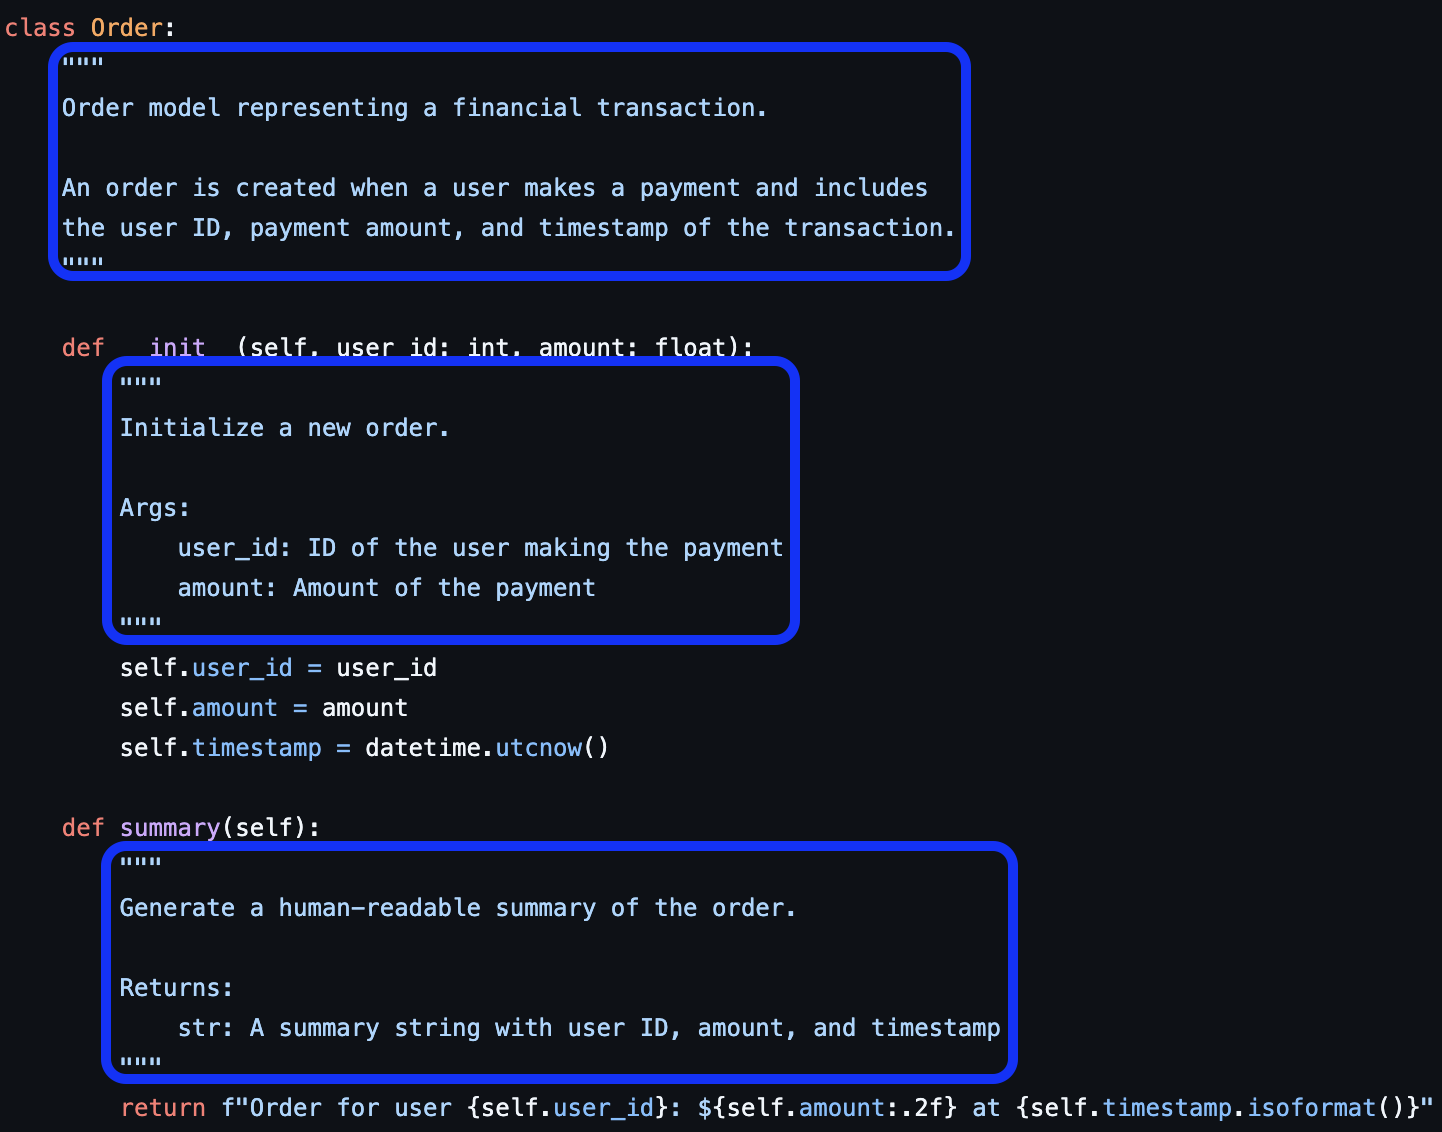
\includegraphics[width=0.8\linewidth]{imgs/png/docstrings.png}
    \caption{Example of Docstrings}
    \label{fig:ex_docstrings}
\end{figure}
